%Anexos

\section{Anexos}\label{sec:anexos}


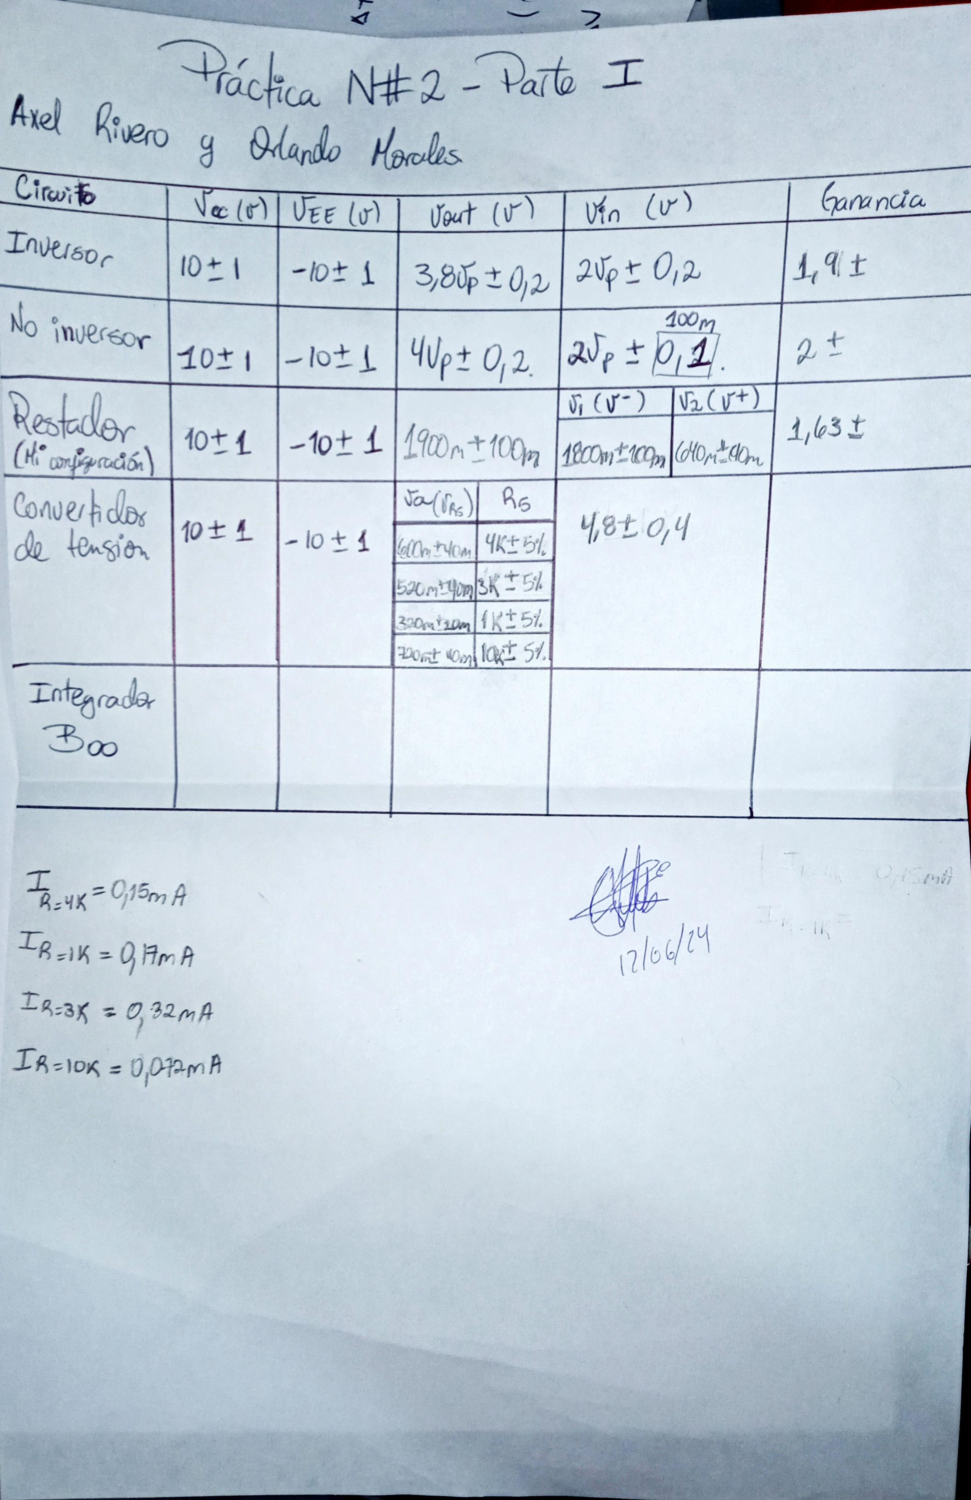
\includepdf[pages=- scale=0.9, fitpaper=true]{pdf/P2 Hoja de datos 1 (2).pdf}
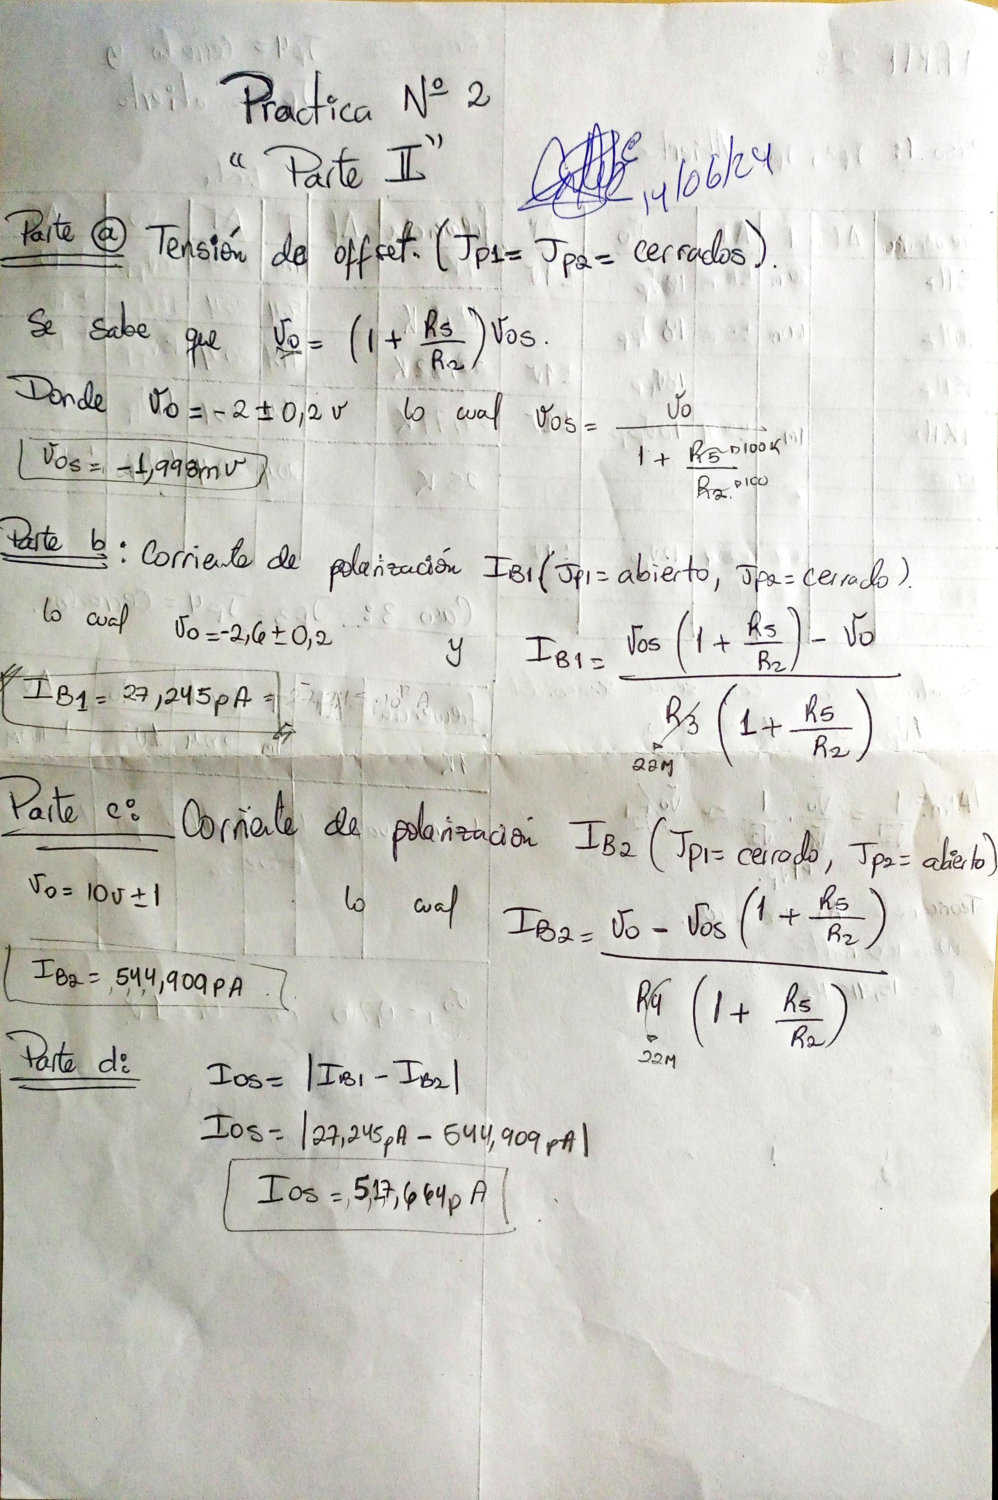
\includepdf[pages=- scale=0.9, fitpaper=true]{pdf/P2 Hoja de datos 2.pdf}
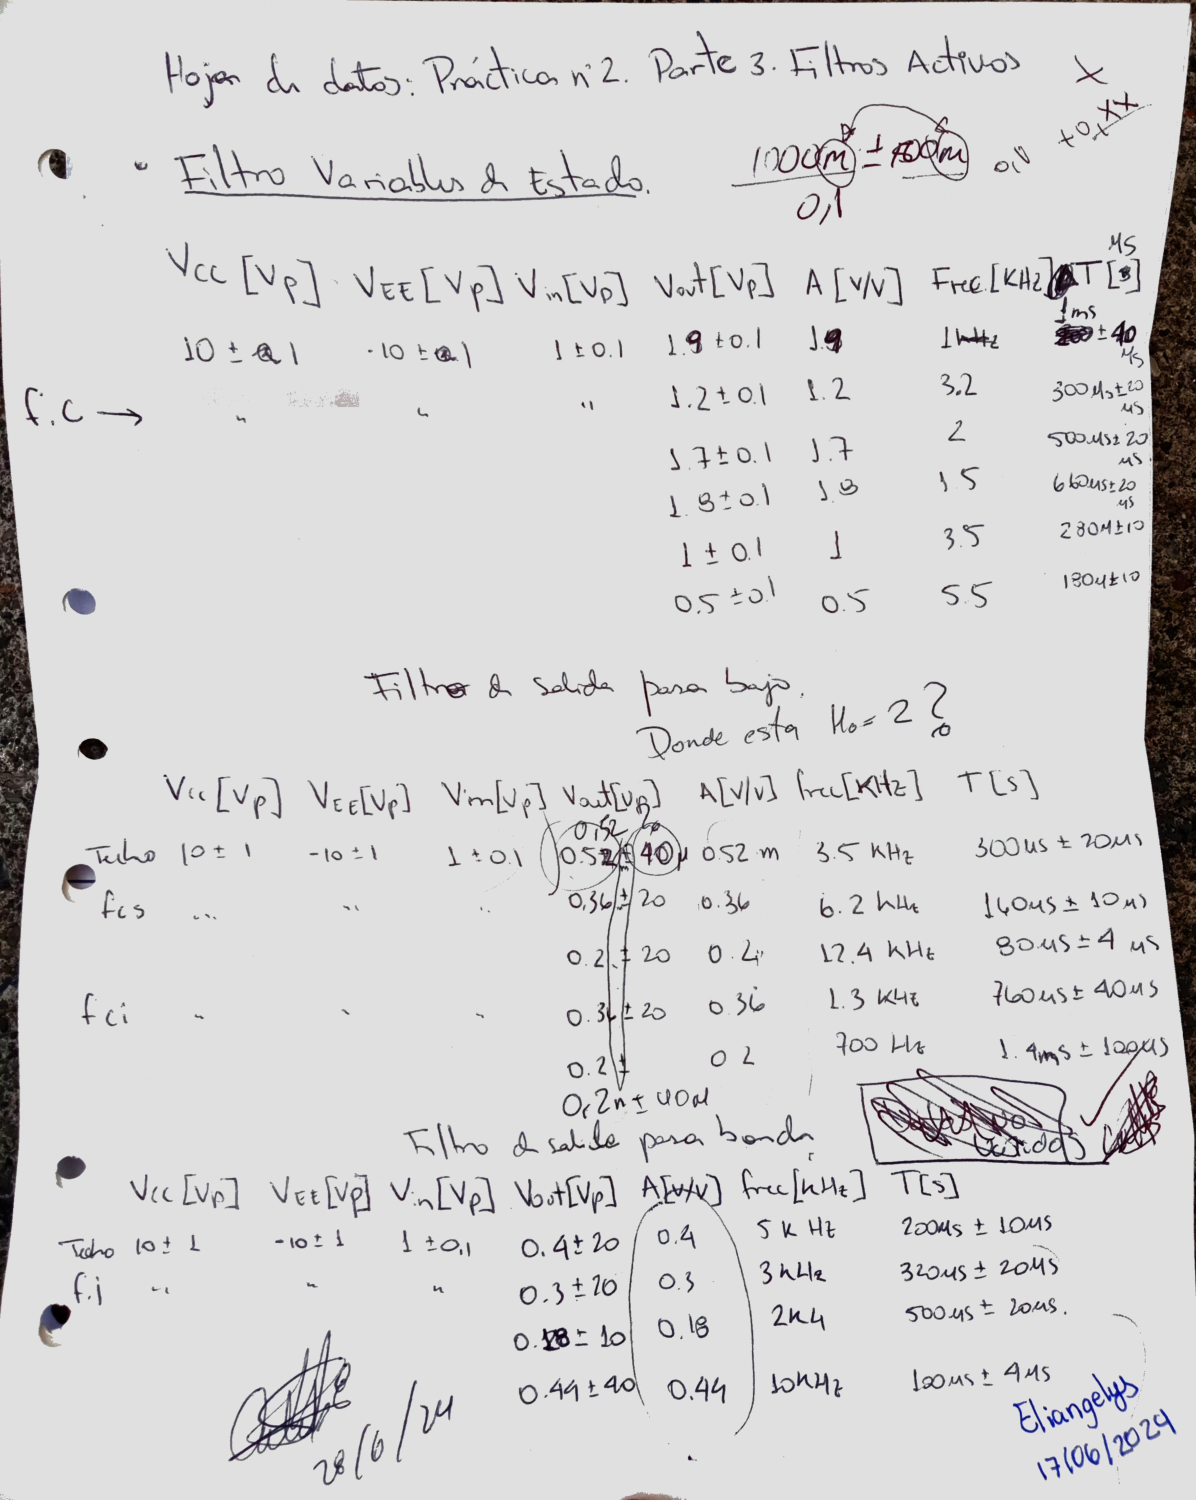
\includepdf[pages=- scale=0.9, fitpaper=true]{pdf/Hoja de datos 3 P2.pdf}
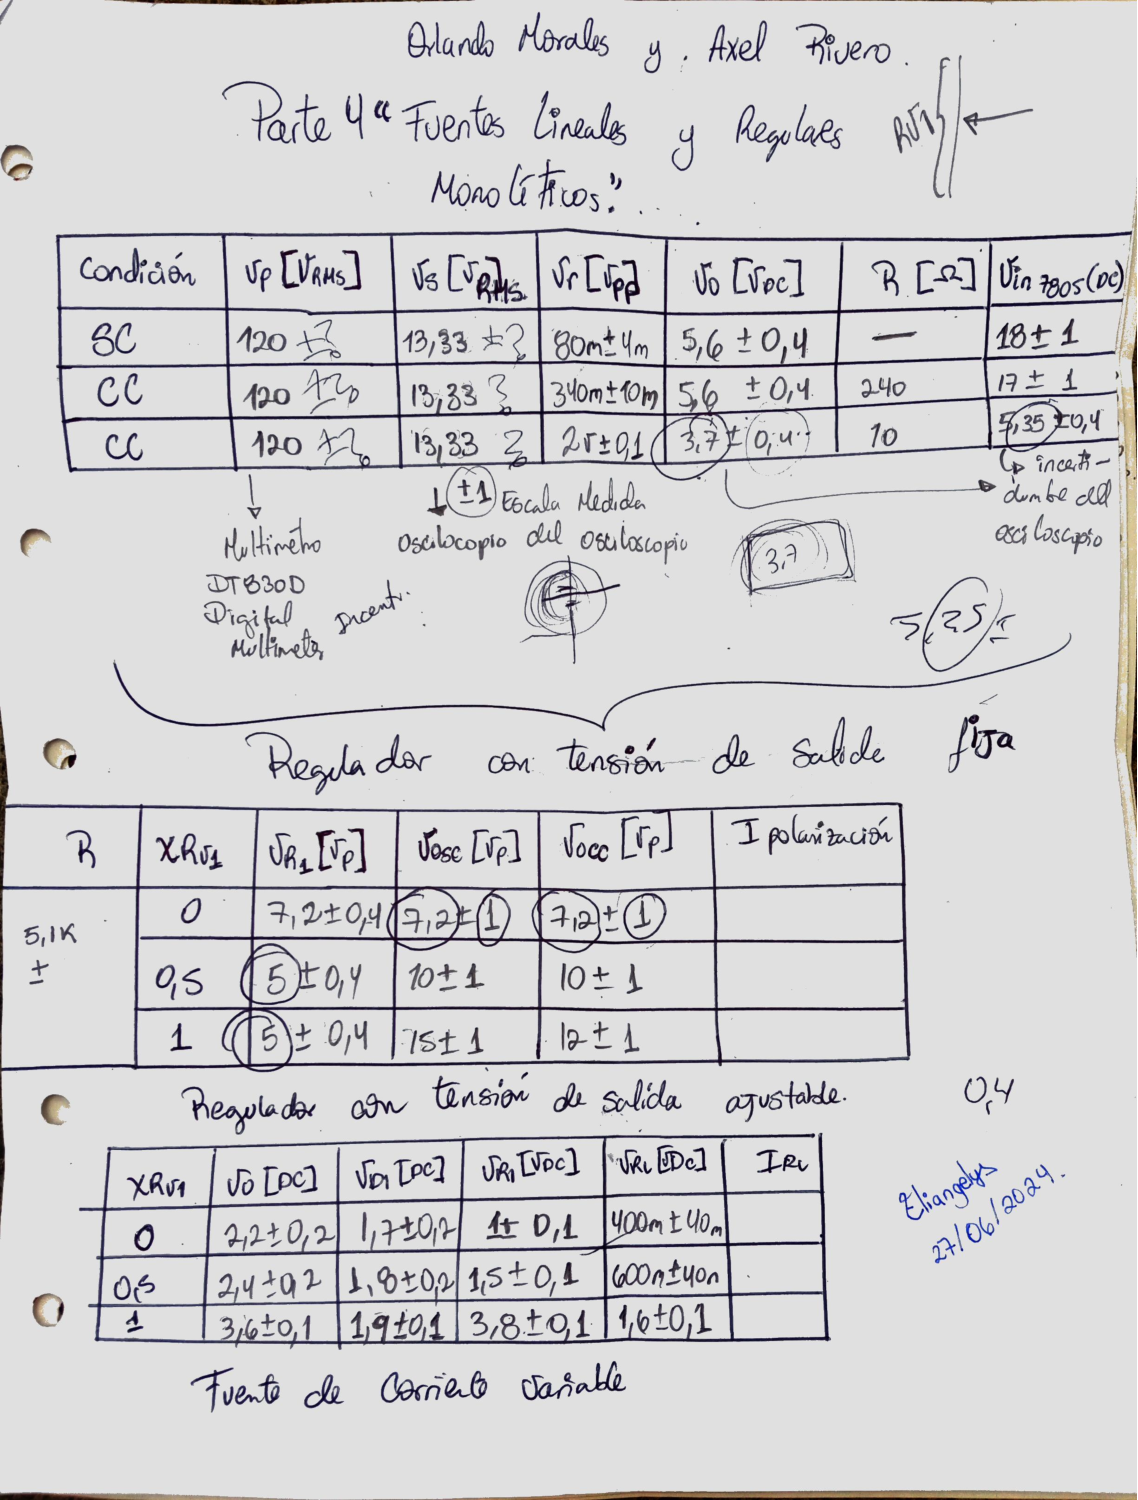
\includepdf[pages=- scale=0.9, fitpaper=true]{pdf/Hoja de datos 4 P2.pdf}
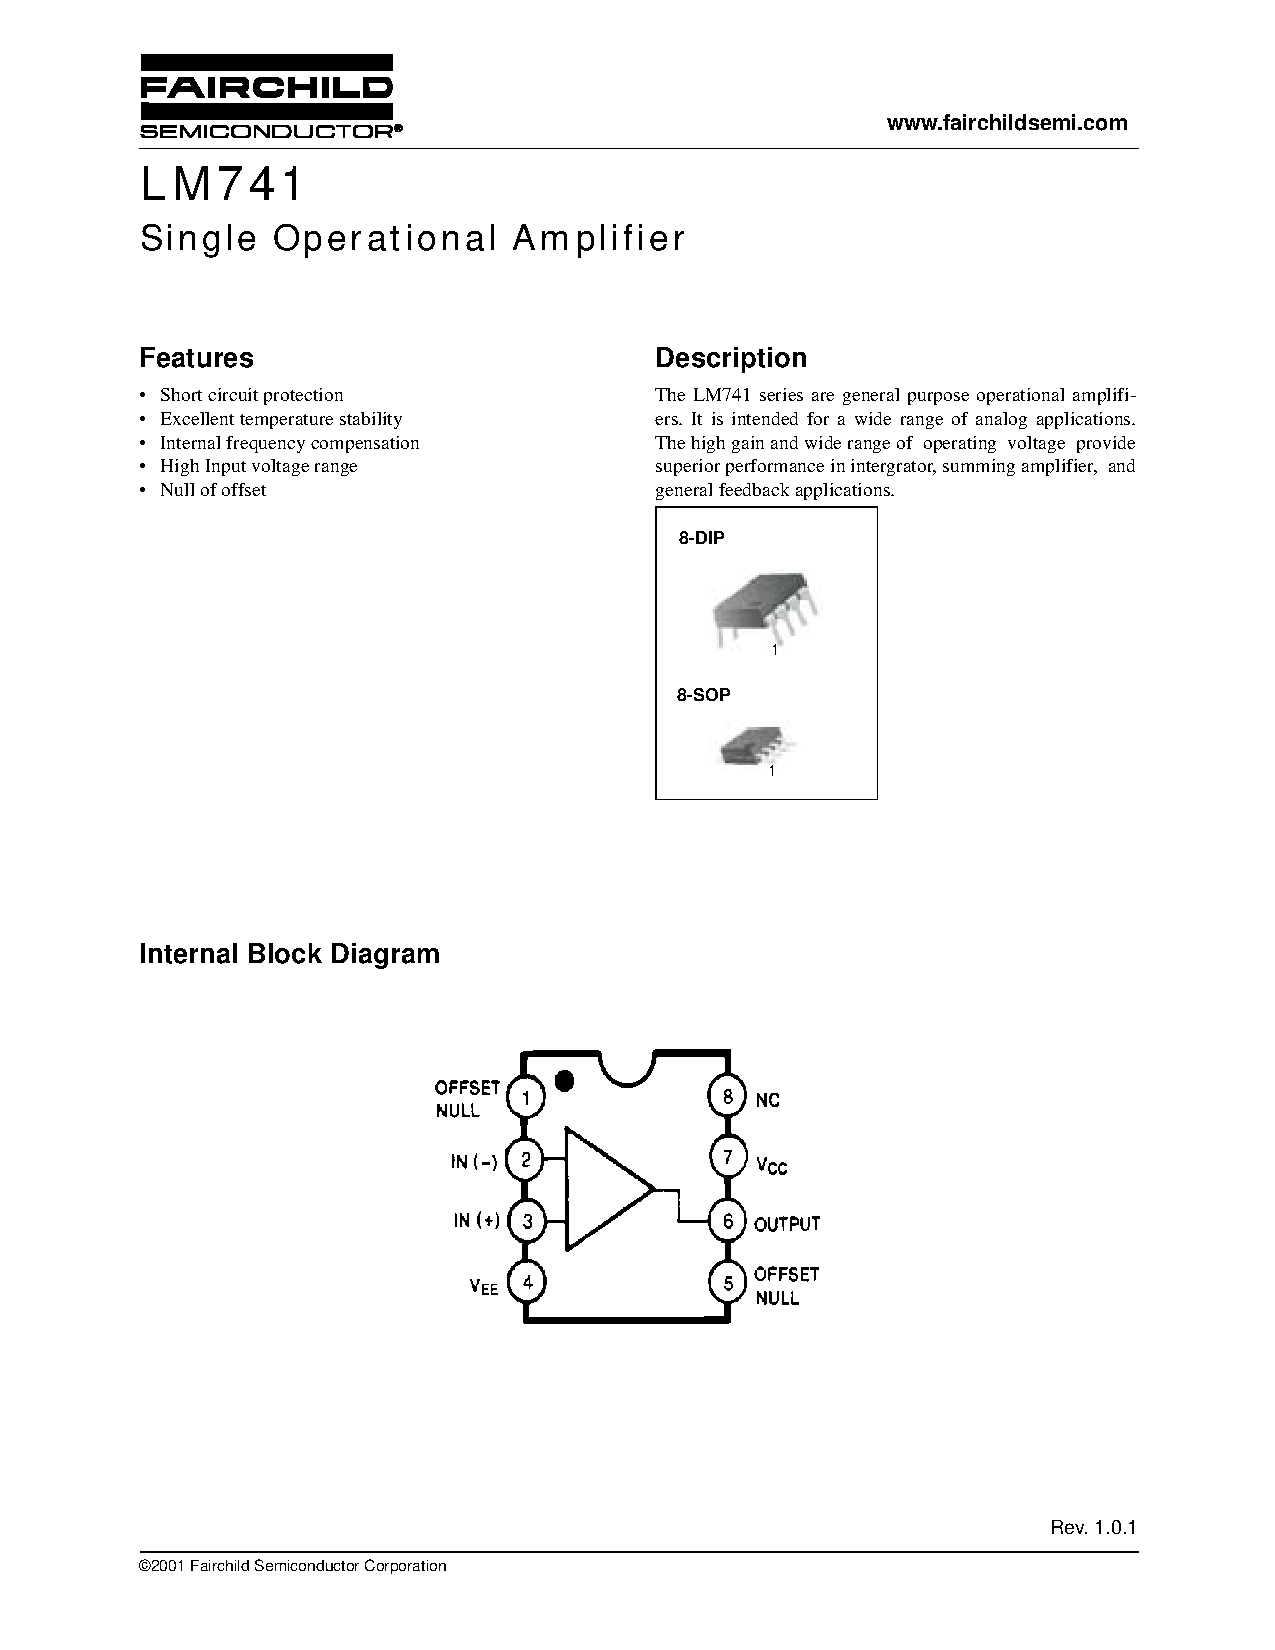
\includepdf[pages=- scale=0.9, fitpaper=true]{pdf/LM741.PDF}
\newpage
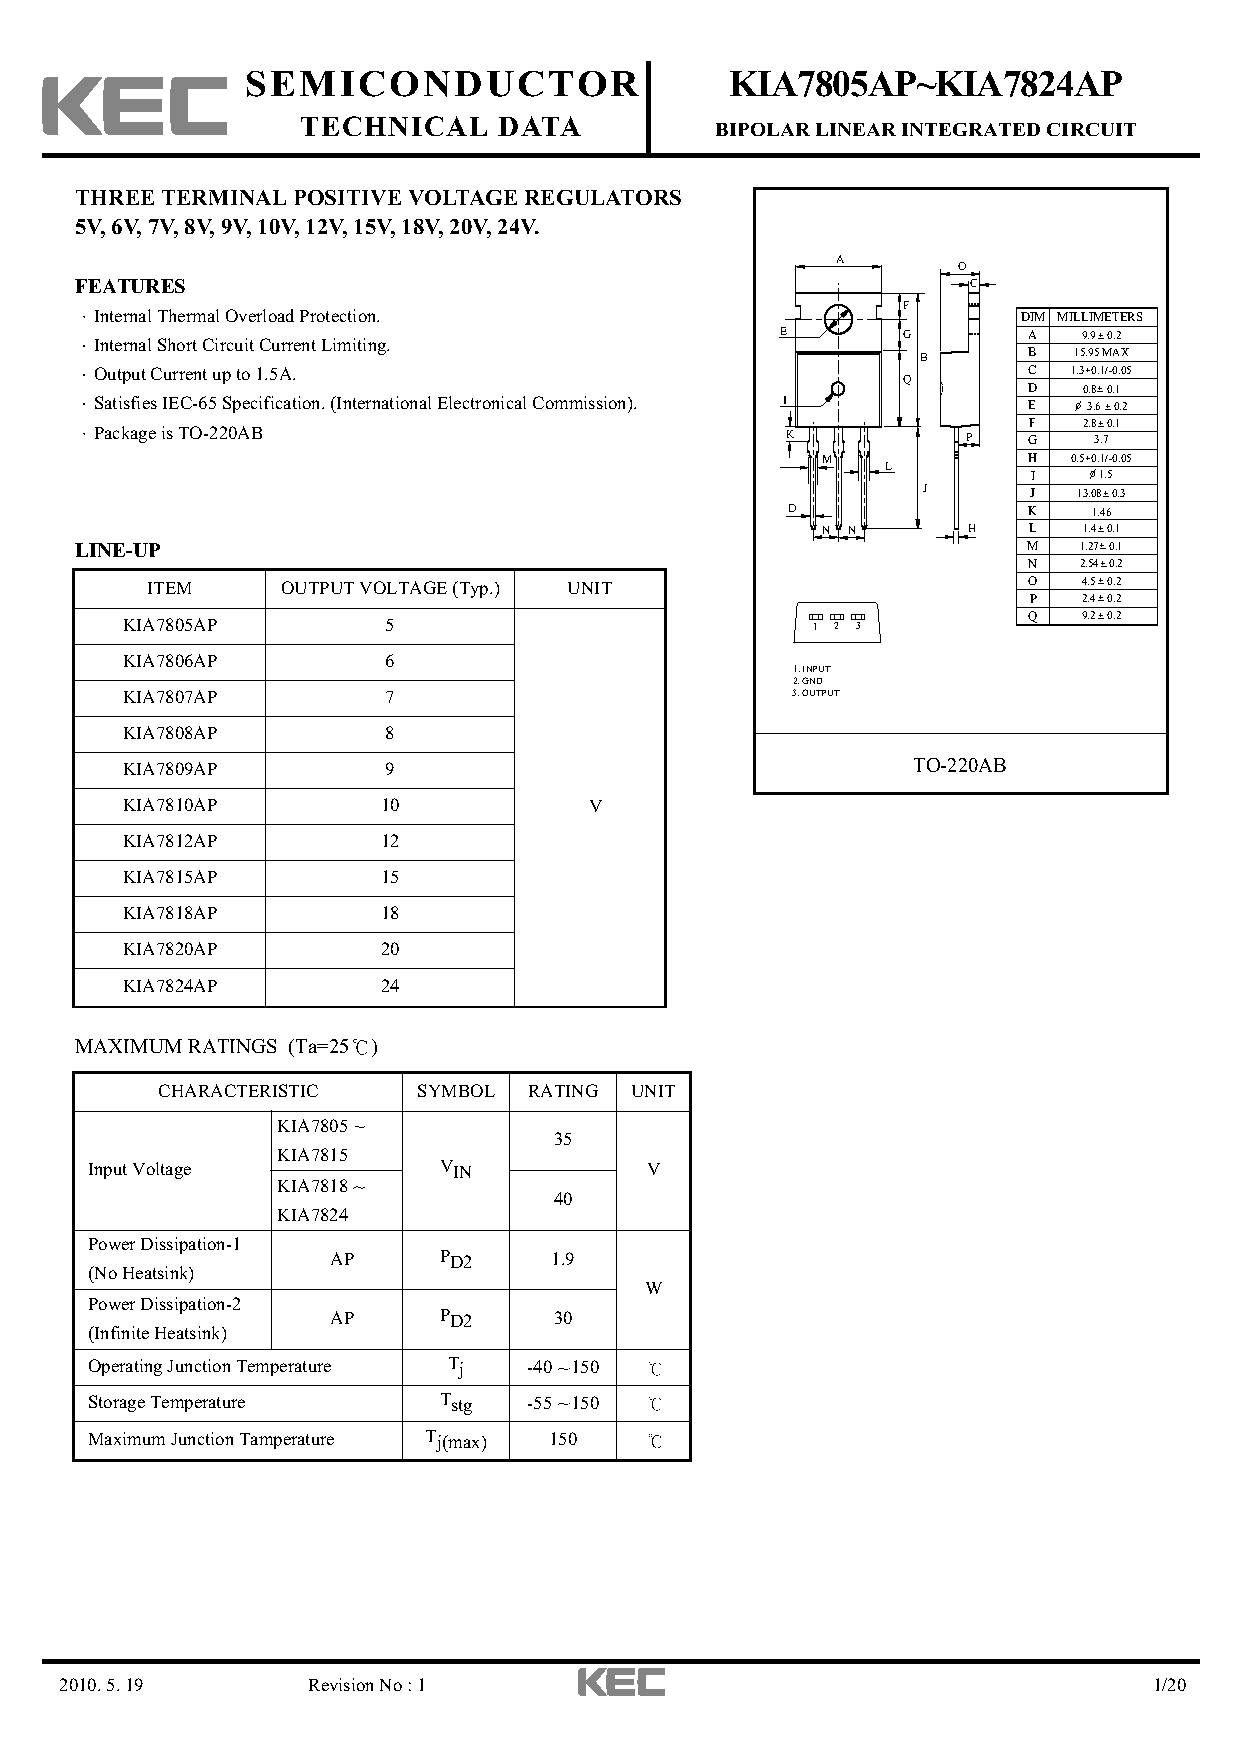
\includepdf[pages=1-3, scale=0.8, fitpaper=true]{pdf/KIA7805AP.PDF}
\includepdf[pages=14-20, scale=0.8, fitpaper=true]{pdf/KIA7805AP.PDF}
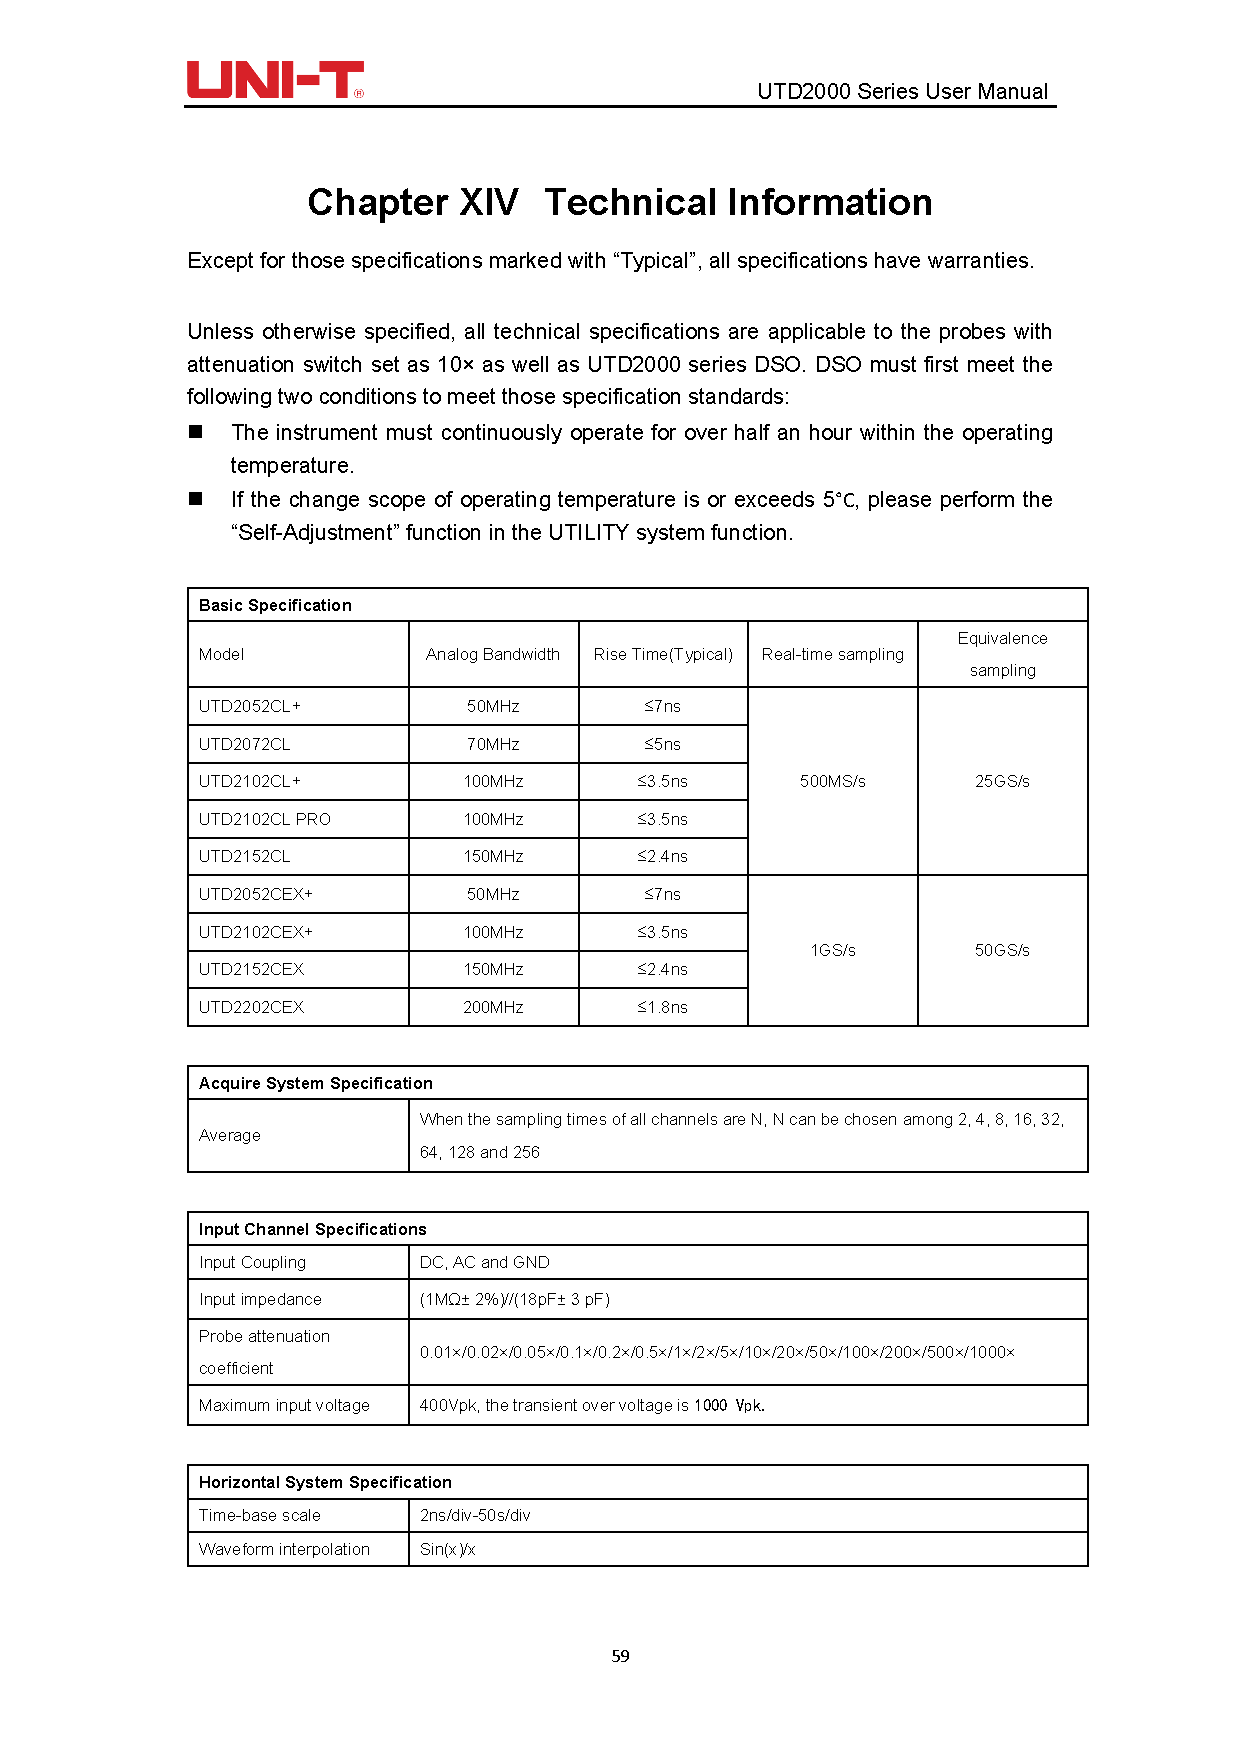
\includepdf[pages=-, scale=0.9,fitpaper=true]{pdf/utd2000_series-001.pdf}
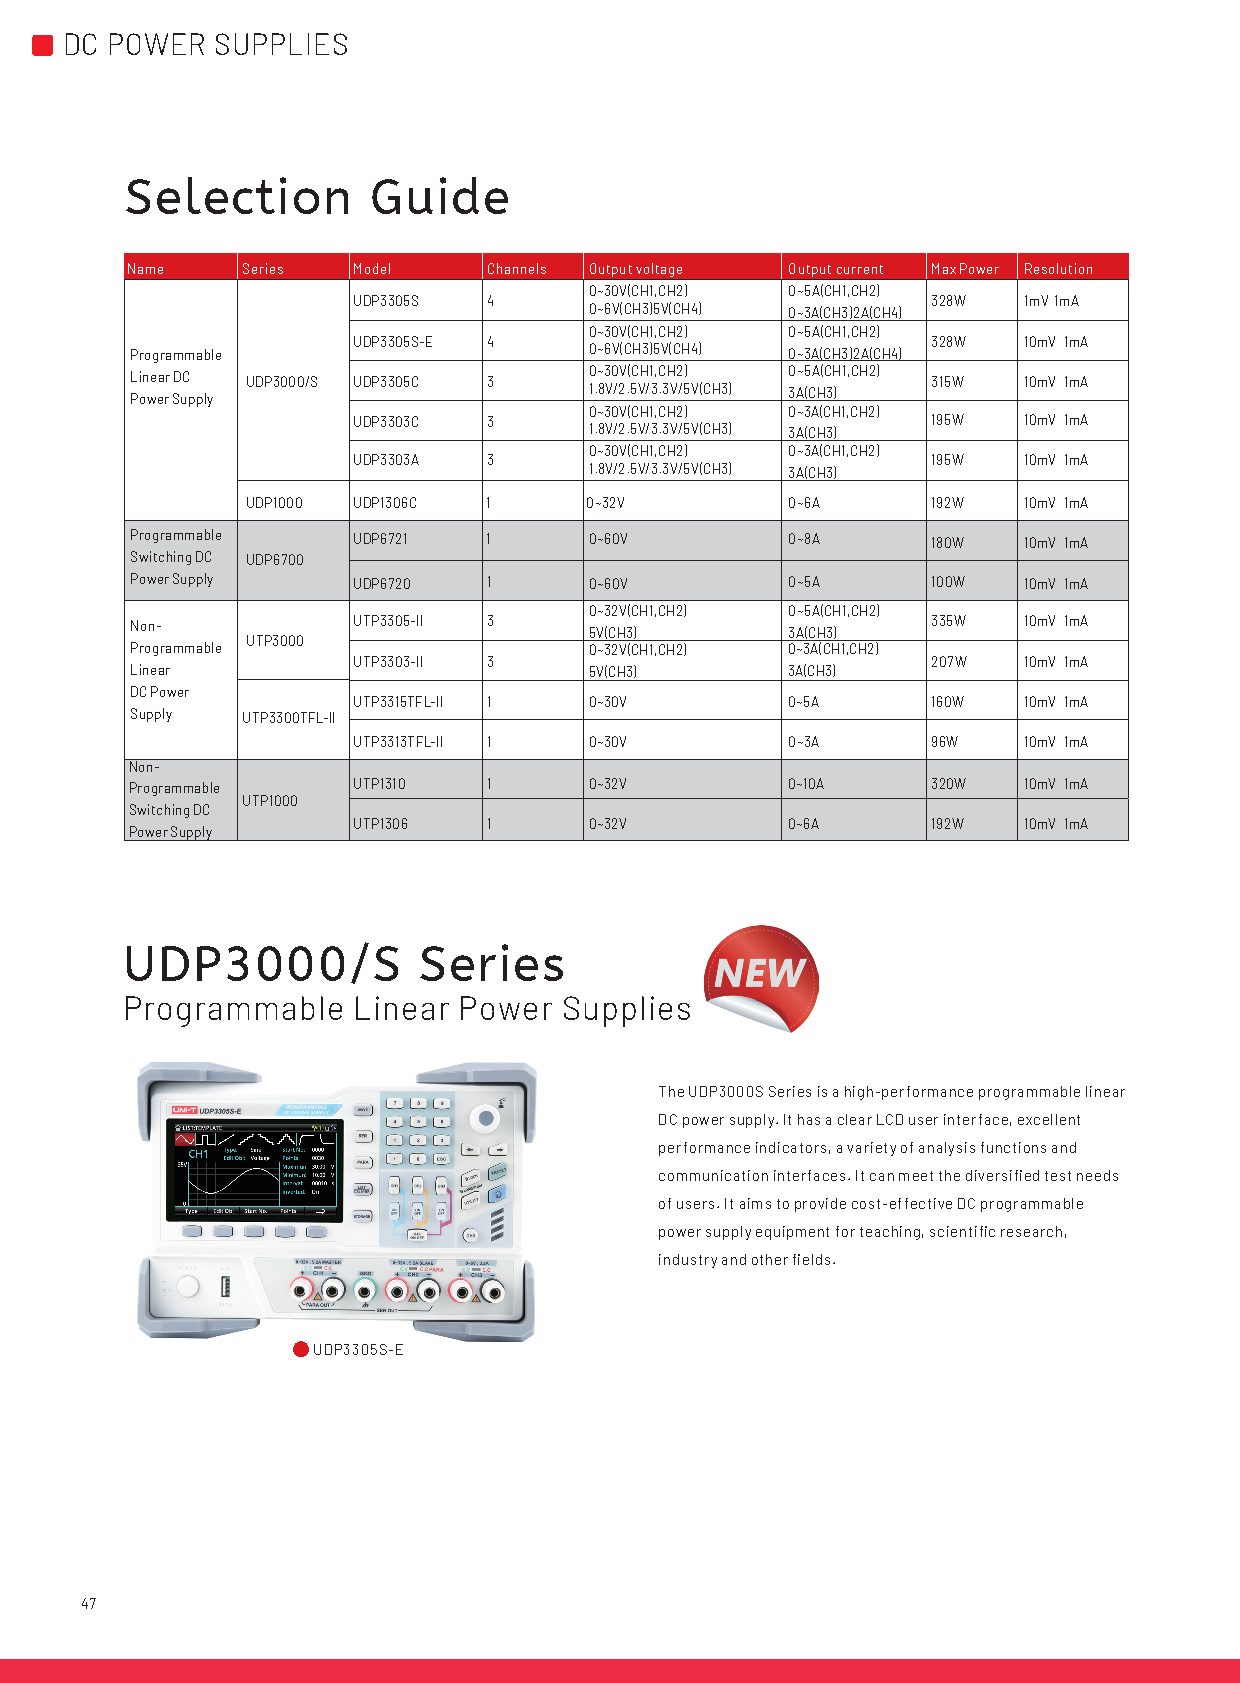
\includepdf[pages=-, scale=0.8, fitpaper=true]{pdf/UTP3305-II.pdf}
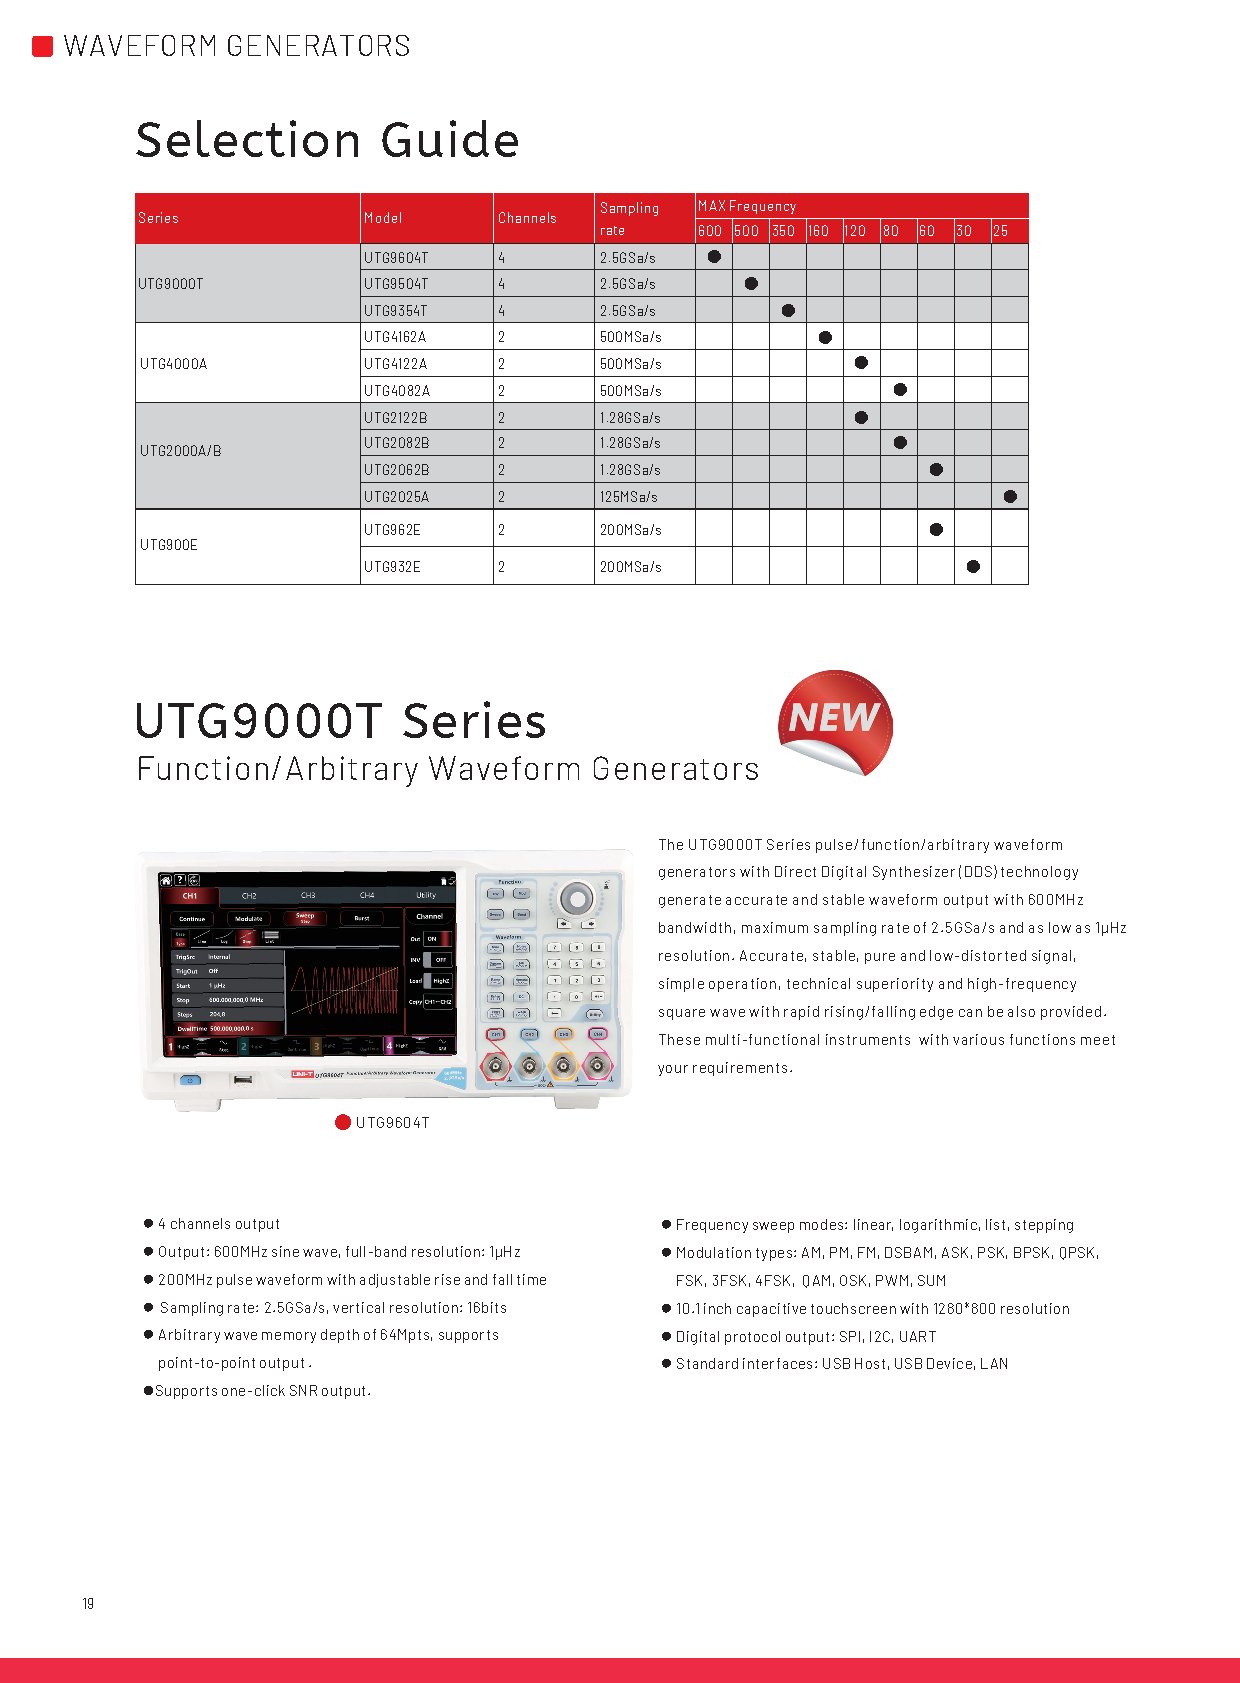
\includepdf[pages=-, scale=0.8, fitpaper=true]{pdf/UTG932E.pdf}

\begin{figure}[H]
    \centering
    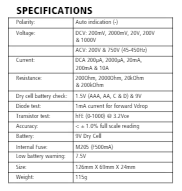
\includegraphics[width=8cm]{Imagenes/DT830D.png}
    \label{eq:DT830D}
\end{figure}

\subsection{Códigos de Octave}\label{subsec:cod_octave}
    \begin{itemize}
        \item Comparación de puntos
            
                \lstinputlisting[language=Octave,basicstyle=\small, caption={Código Octave para análisis de puntos}, label=lst:comparacion]{Scripts/comparacion_puntos.m}
\newpage                
        \item Diagrama asintótico de Bode
            
                \lstinputlisting[language=Octave,basicstyle=\small, caption={Código Octave para análisis de puntos}, label=lst:resp.frecuencia]{Scripts/resp_frecuencia.m}
    \end{itemize}
\newpage